\documentclass[10pt]{article}
\usepackage[polish]{babel}
\usepackage[utf8]{inputenc}
\usepackage[T1]{fontenc}
\usepackage{graphicx}
\usepackage[export]{adjustbox}
\graphicspath{ {./images/} }

\title{LIGA MATEMATYCZNA \\
 PÓŁFINAE \\
 16 lutego 2012 \\
 SZKOŁA PODSTAWOWA }

\author{}
\date{}


\begin{document}
\maketitle
\section*{ZADANIE 1.}
Trzy kolejne liczby trzycyfrowe zapisano obok siebie, bez odstępów, otrzymując liczbę dziewięciocyfrową podzielną przez 4 i 25 . Znajdź te liczby wiedząc, że w ich zapisie dziesiętnym występują jedynie trzy różne cyfry.

\section*{ZADANIE 2.}
Każdy uczeń pewnej klasy sportowej uprawia żeglarstwo, pływanie lub judo. Tylko dwóch uczniów uprawia wszystkie te dyscypliny sportu. Judo i żeglarstwem zajmuje się czworo uczniów. Dziesięciu uprawiających pływanie nie zajmuje się żeglarstwem. Pięciu uprawia pływanie i judo. Żeglarstwem pasjonuje się 19 uczniów. Pływanie i żeglarstwo to dyscypliny uprawiane przez 8 uczniów. Ilu uczniów uprawia judo w tej klasie, skoro wszystkich uczniów jest 36? Ilu uczniów uprawia tylko jedną dyscyplinę sportu?

\section*{ZADANIE 3.}
Ola, Basia, Ewa i Kasia wybrały się na grzyby. Ola i Basia zebrały razem 40 grzybów, Ewa i Kasia 42, a Ola i Kasia 30 grzybów. Ile grzybów zebrały łącznie Basia i Ewa?

\section*{ZADANIE 4.}
Rozpoczynając od pewnej liczby naturalnej, wypisano pięć kolejnych jej wielokrotności. Suma trzech najmniejszych jest równa 33330. Oblicz sumę trzech największych.

\section*{ZADANIE 5.}
Prostokąt został podzielony na kwadraty jak na rysunku. Pole kwadratu zaznaczonego ciemnym kolorem jest równe 1. Wyznacz długości boków wszystkich kwadratów oraz oblicz pole tego prostokąta.\\
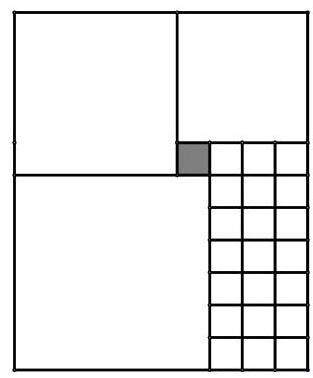
\includegraphics[max width=\textwidth, center]{2024_11_21_999f692427d726960eb3g-1}


\end{document}